\documentclass{ctexart}
\usepackage{PhysicalChemistryNote}

\begin{document}\pagestyle{plain}
\noindent\tbf{\LARGE 7E 温度对反应速率的影响}\vspace{15pt}\\
\indent 实验表明,大多数化学反应的速率总是随着温度升高而增加.我们将从理论上对此给出解释,%
并说明速率常数与温度满足的关系.在本节的最后,我们也将介绍一种测定速率常数的重要办法.\vspace{12pt}\\
\Section{7E.1 Arrhenius方程}
\indent Arrhenius研究了许多气相反应的速率,由此揭示了反应的速率常数与温度的关系.
\begin{theorem}[7E.1.1 Arrhenius方程]
    反应速率常数$k$与温度$T$满足
    \[k=A\exp\left(-\dfrac{E_a}{RT}\right)\]
    其中$A$为\tbf{指前因子},$E_a$为\tbf{表观活化能}.
\end{theorem}
尽管Arrhennius得出的$A$和$E_a$是完全经验性的,但他还是对此做出了一些合理的解释.%
他认为,并不是反应分子的每次接触都能发生反应,只有那些能量足够高的分子之间的角度合适的碰撞才能发生反应.%
这些分子被称为\tbf{活化分子},而由非活化分子变为活化分子所需要的平均能量即为\tbf{(表观)活化能}.%
由上面的定性解释,以及我们在\tbf{1B}中提到的能量分布公式,我们可以简单地推导Arrhenius方程.
\begin{derivation}
    假定能量不低于$E_{\min}$的分子才能发生反应.根据\tbf{1B.3.3},这样的分子占总体的比例为
    \[p=\exp\left(-\dfrac{E_{\min}}{k_\text{B}T}\right)\]
    令$E_a=\NA E_{\min}$.如果活化能$E_a=0$,那么每一次碰撞都会发生反应.%
    不妨记此时$k=A$,这样指前因子$A$就代表每次碰撞都发生反应时对应的速率常数.%
    当$E_a>0$时,能发生反应的分子数的比例变为$p$,那么就有
    \[k=Ap=A\exp\left(-\dfrac{E_a}{RT}\right)\]
    这个推导过程相当粗糙,因而(几乎)只起到定性的作用.
\end{derivation}
对Arrhenius方程取对数后可得
\[\ln k=\ln A-\dfrac{E_a}{RT}\]
如果$A$与$T$无关,就可以通过$\ln k$对$\dfrac1T$作图的方式确定$A$与$E_a$.我们将上式对$T$微分可得
\[\left(\dfrac{\di\ln k}{\di T}\right)=\dfrac{E_a}{RT^2}\]
这可以作为活化能的正式定义.
\begin{definition}[7E.1.2 表观活化能]
    表观活化能$E_a$可以定义为
    \[E_a=RT^2\left(\dfrac{\di\ln k}{\di T}\right)\]

\end{definition}
对于$E_a$不随$T$变化的情形,这就与前面给出的直线等价.%
而$E_a$随$T$变化则可能暗示着反应机理的改变.\\
\indent 对于复杂反应而言,总的表观活化能可以根据反应的速率方程和各基元反应的表观活化能得出.%
例如我们在前面提到的\ce{H2}与\ce{Cl2}的反应,其速率方程为
\[v=\dfrac{1}{2}\dfrac{\di\con{HCl}}{\di t}=k_2\sqrt{\dfrac{k_1}{k_{-1}}}\con{H2}\con{Cl2}^{\frac12}\]
因此表观速率常数$k_{\text{obs}}=k_2\sqrt{\dfrac{k_1}{k_{-1}}}$.于是
\[E_{a,\text{obs}}=A_2\sqrt{\dfrac{A_1}{A_{-1}}}\left(E_{a,2}+\dfrac12E_{a,1}-\dfrac12E_{a,-1}\right)\]
需要注意的是,两个自由基反应形成分子的活化能几乎为$0$,因为自由基本来就是活泼的,只要相遇几乎都能发生反应,%
因此$E_{a,-1}\approx0$.这样,上式也可以改写为
\[E_{a,\text{obs}}=A_2\sqrt{\dfrac{A_1}{A_{-1}}}\left(E_{a,2}+\dfrac12E_{a,1}\right)\]
\begin{theorem}[7E.1.3 自由基偶联反应的表观活化能]
    两个自由基偶联的反应的表观活化能$E_a$近似为$0$.
\end{theorem}
\vspace{8pt}
\Section{7E.2 过渡态理论}
\indent 虽然Arrhenius方程的确能够描述温度对反应的影响,可它毕竟是定性的,%
并没有很好地在微观层面解释反应的机制,也没有合适的理论证明其成立性.%
为了填补这一空白,Eyring等人提出了\tbf{过渡态理论},揭示了反应发生的具体过程.\vspace{4pt}\\
\Part{势能面,反应坐标与过渡态}
\indent 我们设想发生反应的是\ce{A}与\ce{B}两个分子.它们的原子分别为$\ce{A}_1,\cdots,\ce{A}_j$和$\ce{B}_1,\cdots,\ce{B}_k$.%
显然,这两个分子构成的系统的能量会随着\ce{A}与\ce{B}的相对发生变化.我们不妨用函数表示体系的能量,即
\[E=f\left(\li{\ce{A}},j,\li{\ce{B}},k\right)\]
这一函数接受所有$j+k$个原子的位置为自变量,并给出总能量\footnote{这里指势能.}$E$.%
在实际应用中,通常也会使用各个原子之间的距离$d$,键角$\theta$等参数描述原子的相对位置,%
并作为$E$的自变量.我们把系统处于某一状态下的位置信息统一为一个元素$S$,这样就有$E=f(S)$.%
所有可能的$S$组成了一个集合$X$,$X$内的任意元素都代表了各个原子的一种位置状态.
\begin{definition}[7E.2.1 势能面]
    \tbf{势能面}即表示某一微观体系的势能和相关参数(通常为原子坐标)之间的函数关系,是势能函数$E=f(S)$的图像.
\end{definition}
\indent 如果$S$是一维的,这意味着我们可以在二维平面上画出$E-S$图(正如一般的一元函数一样,这是一条曲线).%
类似地,如果$S$是二维的,就可以在三维空间中画出$E-S$的图像,这则是一片曲面.当$S$的维度更高时,%
直观上并没有$E-S$图的很好的几何对应,但其数学意义仍然是清晰的.\\
\indent 如果\ce{A}与\ce{B}发生了反应生成产物\ce{P},那么上面的集合$X$中也应当有元素$S_{\ce{P}}$,以对应所有原子组成\ce{P}的状态.%
$S_{\ce{P}}$可以从\ce{P}的结构直接得到.我们再考虑\ce{A}和\ce{B}距离足够远的状态$S_{\ce{A}+\ce{B}}$作为反应的起始状态.\\
\indent 现在,我们只需要考虑系统如何由状态$S_{\ce{A}+\ce{B}}$变为$S_{\ce{P}}$即可.%
你可以认为\ce{A}和\ce{B}都分解为独立的原子之后再组合成\ce{P},不过那样的方式太过粗暴,%
并且显然会消耗不少的能量.\ce{A}和\ce{B}会明智地选择一种能量最低的方式变成\ce{P}%
\footnote{如果我们从能量分布的角度考虑此事,就会发现能量更高的途径对应的概率更低,因此过于高能的中间状态事实上出现的概率非常小,因此不纳入考虑中.%
而系统发生变化的途径最有可能的途径正是能量最低的途径.},%
即反应发生的真实途径.我们把这一途径称为\tbf{反应坐标}.
\begin{definition}[7E.2.2 反应坐标]
    \tbf{反应坐标}(reaction coordinate)是由反应物变为产物的过程中系统状态的集合,%
    也对应势能面上连接反应物和产物的最低能量路径.
\end{definition}
反应坐标准确地描述了反应进行的过程.例如,对于\ce{A + B -> P}这一反应,系统能量与反应坐标可能具有下面的关系.
\begin{figure}[H]
    \centering\documentclass{standalone}
\usepackage{PhysicalChemistryNote}
\begin{document}
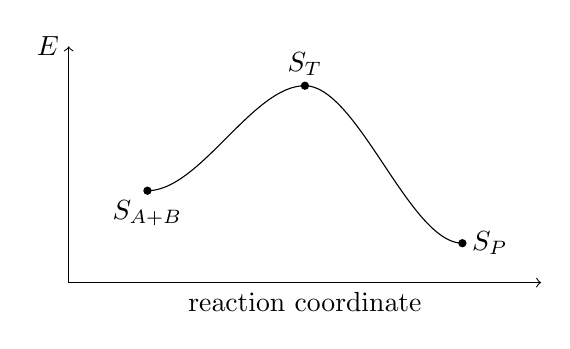
\begin{tikzpicture}
    \draw[->] (0,0)--(6,0) ;
    \node[below] at (3,0) {reaction coordinate};
    \draw[->] (0,0)--(0,3) node[left]{$E$};
    \draw[domain=1:3] plot[smooth] (\x,{(-(\x-2)^3+3*\x-0.5)/3});
    \draw[domain=3:5] plot[smooth] (\x,{((\x-4)^3-3*\x+15)/2});
    \fill (1,7/6) circle (1.5pt) node[below]{$S_{\ce{A}+\ce{B}}$};
    \fill (3,2.5) circle (1.5pt) node[above]{$S_{\ce{T}}$};
    \fill (5,0.5) circle (1.5pt) node[right]{$S_{\ce{P}}$};
    
\end{tikzpicture}
\end{document}
\end{figure}
这正是我们限制$S$在反应坐标内后得到的势能面的截面.%
并且,这条曲线的最高点对应的状态$S_{\ce{T}}$具有如下的性质.
\begin{definition}[7E.2.3 过渡态]
    \tbf{过渡态}是反应坐标中能量的最高点对应的系统状态.%
\end{definition}
\begin{theorem}[7E.2.4 过渡态的数学意义]
    过渡态是整个势能面的\tbf{鞍点}.在这一点,只有沿着反应坐标的方向变化,势能才会降低,%
    除此之外的任意方向都会使得势能升高.
\end{theorem}
下图中的中心点就是鞍点的示意.如果我们要从前面这一侧翻越到后面这一侧,那么能量最低的选择就是通过鞍点.
\begin{tightcenter}
    \documentclass{standalone}
\usepackage{PhysicalChemistryNote}
\begin{document}
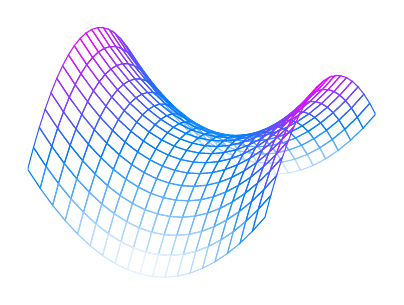
\begin{tikzpicture}
    \begin{axis}[
        hide axis,
        width=6cm,
        height=6cm,
        colormap/cool
    ]
    \addplot3[
        mesh,
        samples=20,
        domain=-1:1,
    ]
    {x^2-y^2};
    \end{axis}
\end{tikzpicture}
\end{document}
\end{tightcenter}
想象一下,你打算翻过一座山.这座山恰好有一个山坳,因此你就决定从那里过去,%
而不会傻乎乎地先爬到山顶再下山.这个山坳就是上图中的鞍点.
\begin{hint}
    作为补充,在数学上,我们通过计算Hessian矩阵判断鞍点,在鞍点处的Hessian矩阵仅有一个负本征值,对应反应坐标方向.这也是计算化学中寻找过渡态的重要依据.
\end{hint}

\indent 过渡态的物理意义在于它描述了反应物到产物的中间状态,即旧键将断未断,新键将成未成的状态.%
这一状态也被称作\tbf{活化络合物}.这需要与中间体区分.\vspace{4pt}\\
\Part{过渡态理论与Eyring方程}
\indent 我们已经找到了一种十分优秀的描述反应过程的方式,而我们并不打算止步于此.%
在做出过渡态理论的基本假设后,我们可以给出活化能的更明确的定义,并据此得出过渡态理论中的一个重要公式.
\begin{theorem}[7E.2.5 过渡态理论的基本假设]
    \begin{enumerate}[topsep=0pt,parsep=0pt,itemsep=0pt,partopsep=0pt,label=\tbf{\arabic*.},leftmargin=*]
        \item 反应物变为产物的过程总是经过势能面上的鞍点,即过渡态.
        \item 反应物和过渡态(活化络合物)总是处于准平衡态.
        \item 过渡态向产物的转化是不可逆的.
        \item \tbf{2.}和\tbf{3.}的反应也满足质量作用定律.
    \end{enumerate}
\end{theorem}
我们也可以将后两点假设表示为下面的过程.
\begin{tightcenter}
    \ce{A + B <=> T$^\ddagger$ -> P}
\end{tightcenter}
现在我们来推导描述反应速率常数的方程.
\begin{derivation}\setcounter{equation}{0}
    考虑实际反应
    \begin{tightcenter}
        \ce{A + B ->T[$k$] P}
    \end{tightcenter}
    以及过渡态\ce{T$^\ddagger$}向产物\ce{P}的转化反应
    \begin{tightcenter}
        \ce{T$^\ddagger$ ->T[$k^\ddagger$] P}
    \end{tightcenter}
    根据基本的动力学假设,我们可以得到
    \begin{equation}
        \dfrac{\di\con{P}}{\di t}=k\con{A}\con{B}=k^\ddagger\con{T^\ddagger}
    \end{equation}
    于是第一步平衡的平衡常数
    \begin{equation}
        K=\dfrac{\con{T^\ddagger}}{\con{A}\con{B}}=\dfrac{k}{k^\ddagger}
    \end{equation}
    活化络合物转化为产物的速率常数与活化络合物中的振动有关,这一振动使得活化络合物更类似于产物,从而使得活化络合物沿着反应坐标向产物方向倾斜.%
    我们把振动频率记为$\nu$.\\
    然而,不是所有振动都可以使得过渡态向产物的方向转化.分子中的其他原子可能并不能够适当地排列以使过渡态转化为产物,%
    或者分子的旋转状态妨碍了过渡态向产物的转变.只有一部分的振动可以使得我们希望的转化发生,因此我们定义\tbf{传递系数}$\kappa$表示这样的振动的所占的比例.于是就有
    \begin{equation}
        k^\ddagger=\kappa\nu
    \end{equation}
    现在我们来考虑$K$.虽然过渡态并不满足统计力学(它的留存时间太短),但我们可以采取统计力学方法%
    证明它与一个真正的平衡常数$K^\ddagger$成比例关系,即
    \begin{equation}
        K=\left(\dfrac{k_{\text B}T}{h\nu}\right)K^\ddagger
    \end{equation}
    由(2)(4)和(5)可得
    \begin{equation}
        k=Kk^\ddagger=\kappa\left(\dfrac{k_{\text B}T}{h}\right)K^\ddagger
    \end{equation}
    而由$K^\dagger$可以定义活化Gibbs自由能,活化焓和活化熵,即
    \begin{equation}
        \Delta G^\ddagger=-RT\ln K^\ddagger
    \end{equation}
    \begin{equation}
        \Delta G^\ddagger=\Delta H^\ddagger-T\Delta S^\ddagger
    \end{equation}

\end{derivation}
这样,我们就得到了Eyring方程.
\begin{theorem}[7E.2.6 Eyring方程]
    基元反应的速率常数$k$满足
    \[k=\kappa\left(\dfrac{k_\text BT}{h}\right)\exp\left(-\dfrac{\Delta G^\ddagger}{RT}\right)\]
    其中$\kappa$为\tbf{传递系数},$\Delta G^\ddagger$为活化Gibbs自由能.
\end{theorem}
我们可以改写Eyring方程得到
\[k=\left[\kappa\left(\dfrac{k_\text BT}{h}\right)\exp\left(\dfrac{\Delta S^\ddagger}{R}\right)\right]\exp\left(-\dfrac{\Delta H^\ddagger}{RT}\right)\]
如果假定$\Delta H^\ddagger$不随温度变化,那么对于基元反应,这就是Arrhenius方程的形式,其中
\[A=\kappa\left(\dfrac{k_\text BT}{h}\right)\exp\left(\dfrac{\Delta S^\ddagger}{R}\right)\ \ \ \ \ E_a=\Delta H^\ddagger\]
因此,可以认为指前因子$A$主要由活化熵$\Delta S^\ddagger$决定,而活化能$E_a$主要由活化焓$\Delta H^\ddagger$决定.\\
\indent 过渡态理论比起传统的碰撞理论是对反应过程描述的一大进步.%
它通过活化络合物模型,成功将分子动力学与宏观反应速率结合,并且为计算化学提供了%
计算反应速率的理论基础.
\begin{hint}
    如果你感到上面的内容模糊不清,并且想详细了解过渡态理论的相关内容,那么笔者建议你阅读《现代物理有机化学》一书的第七章.%
    顺带一提,这本书的所有内容都非常值得你仔细学习.
\end{hint}
\vspace{8pt}
\Section{7E.3 弛豫法测定速率常数}
\indent 我们在本章的前几节介绍了几种测定速率的简单方法.%
自然,有更加精密和先进的手段测定反应速率,不过我们并不打算介绍那些复杂的仪器与方法,%
而是介绍一种重要的,与速率方程密切相关的测定对峙反应速率常数的方法——\tbf{弛豫法}.
\begin{definition}[7E.3.1 弛豫]
    \tbf{弛豫}是指的是在某一个渐变过程中从某一个状态逐渐地恢复到平衡态的过程.
\end{definition}
对于一个处于平衡的化学反应而言,如果改变温度(这通常通过放电,激光等方式进行),那么平衡将发生移动.%
测定各种物质的浓度随时间的变化,就能获知反应的速率常数.%
我们从最简单的反应\ce{A <=> P}开始.
\begin{derivation}
    系统初始处于平衡态.我们假定改变条件后有
    \begin{tightcenter}
        \ce{A <=>T[$k_1$][$k_{-1}$] P}
    \end{tightcenter}
    并且最终平衡时\ce{A}和\ce{P}的浓度分别为$\con{A}_{\text{eq}}$和$\con{P}_{\text{eq}}$.这样就有
    \[k_1\con{A}_{\text{eq}}=k_{-1}\con{P}_{\text{eq}}\]
    令$x=\con{A}-\con{A}_{\text{eq}}=\con{P}_{\text{eq}}-\con{P}$表示反应偏离平衡的程度,就有
    \[\begin{aligned}
        \dfrac{\di\con{A}}{\di t}
        &= k_{-1}\con{P}-k_1\con{A} \\
        &= k_{-1}\left(\con{P}_{\text{eq}}-x\right)-k_1\left(\con{A}_{\text{eq}}+x\right) \\
        &= -\left(k_{-1}+k_1\right)x+k_{-1}\con{P}_{\text{eq}}-k_1\con{A}_{\text{eq}} \\
        &= -\left(k_1+k_{-1}\right)x
    \end{aligned}\]
    又因为$\dfrac{\di\con{A}}{\di t}=\dfrac{\di x}{\di t}$,于是有
    \[\dfrac{\di x}{\di t}=-\left(k_1+k_{-1}\right)x\]
    这是一个一阶微分方程,其解为
    \[x=x_0\e^{-\left(k_1+k_{-1}\right)t}\]
    其中$x_0$即为初始状态的$x$(亦即条件改变前后平衡状态时$\con{A}$或$\con{P}$之差).我们令弛豫时间$\tau=\dfrac{1}{k_1+k_{-1}}$,就有
    \[x=x_0\e^{-\frac{t}{\tau}}\]
    测定$x$依时间的变化关系,得出弛豫时间$\tau$,再结合平衡常数$K=\dfrac{k_1}{k_{-1}}$就可以得出$k_1$与$k_{-1}$.%
    这为我们测定对峙反应的正逆反应速率常数提供了一个相当不错的办法.
\end{derivation}
对于更复杂的体系,处理方法是类似的.我们以\ce{A + B <=> C + D}为例.
\begin{derivation}
    系统初始处于平衡态.我们假定改变条件后有
    \begin{tightcenter}
        \ce{A + B <=>T[$k_1$][$k_{-1}$] C + D}
    \end{tightcenter}
    同样地,平衡时有
    \[k_1\con{A}_{\text{eq}}\con{B}_{\text{eq}}=k_{-1}\con{C}_{\text{eq}}\con{D}_{\text{eq}}\]
    仍令$x=\con{A}-\con{A}_{\text{eq}}$为反应偏离平衡的程度,于是有
    \[\begin{aligned}
        \dfrac{\di x}{\di t}
        = &\ \dfrac{\di\con{A}}{\di t} = k_{-1}\con{C}\con{D}-k_1\con{A}\con{B} \\
        = &\ k_{-1}\left(\con{C}_{\text{eq}}-x\right)\left(\con{D}_{\text{eq}}-x\right)-k_1\left(\con{A}_{\text{eq}}+x\right)\left(\con{B}_{\text{eq}}+x\right) \\
        = &\ k_{-1}\con{C}_{\text{eq}}\con{D}_{\text{eq}}-k_1\con{A}_{\text{eq}}\con{B}_{\text{eq}} \\
          &\ -\left[k_{-1}\left(\con{C}_{\text{eq}}+\con{D}_{\text{eq}}\right)+k_1\left(\con{A}_{\text{eq}}+\con{B}_{\text{eq}}\right)\right]x \\
          &\ +\left(k_{-1}-k_1\right)x^2
    \end{aligned}\]
    由于我们的条件改变总是很微小的(否则也无法保证条件的改变在一瞬间内完成),因此$x$相对各物质的平衡浓度也是很小的.于是,我们忽略上式的二次项即可得
    \[\dfrac{\di x}{\di t}=-\left[k_{-1}\left(\con{C}_{\text{eq}}+\con{D}_{\text{eq}}\right)+k_1\left(\con{A}_{\text{eq}}+\con{B}_{\text{eq}}\right)\right]x\]
    这也是一个一阶微分方程.对应的弛豫时间为
    \[\tau=\dfrac{1}{k_1\left(\con{A}_{\text{eq}}+\con{B}_{\text{eq}}\right)+k_{-1}\left(\con{C}_{\text{eq}}+\con{D}_{\text{eq}}\right)}\]

\end{derivation}
\begin{theorem}[7E.3.2 弛豫法测定速率常数]
    当反应处于平衡时,给系统一个微小的扰动(例如升高温度),测定体系中物质的浓度偏离新的平衡状态的差值$x$随时间$t$的变化,%
    就可以根据前面的推导过程求出正逆反应的速率常数.
\end{theorem}
\end{document}